\documentclass[12pt,a4paper]{book}
\usepackage[utf8]{inputenc}
\usepackage[T1]{fontenc}
\usepackage{amsmath}
\usepackage{amssymb}
\usepackage{ntheorem}
\usepackage[left=2.54cm, right=2.54cm, top=2.54cm, bottom=2.54cm]{geometry}
\usepackage{graphicx}
\usepackage{svg}
\usepackage{calc}
\usepackage{tcolorbox}
\tcbuselibrary{breakable}
\usepackage[
pdftitle={},
pdfsubject={},
pdfauthor={},
pdfkeywords={},
hidelinks,
colorlinks=true,
allcolors=blue,
]{hyperref}
\usepackage{fancyhdr}
\usepackage{tikz}
\usetikzlibrary{positioning}

\usepackage[
backend=biber,
% language=english
% citestyle=ieee
% maxbibnames=2,
% firstinits=true
backref=true,
refsection=chapter,
]{biblatex}
\bibliography{references.bib}

\usepackage{algorithm}
\usepackage{algpseudocodex}

\begin{document}
	\title{My Lecture Note: Robotics}
	\author{Phayuth}
	\maketitle

	\tableofcontents

	\chapter{Camera Modeling}

This article presents the method of camera modeling and calibration. Projection, Collinearity Model equation, Distortion model, Bundle Adjustment.

\section*{Nomenclature}
\begin{tabbing}
    $P$\qquad \= Projection Matrix\\
    $x$ \> Pixel\\
\end{tabbing}


\section{Camera Model}
\subsection{Projection Model}
A 3D point in the world coordinate is projected onto the image plane using a camera projection matrix. \cite{calibCameraModels}, \cite{opencvCameraCalibration}


\[
s p = K [R |t ] P_w
\]

Here, $P_w$ is a 3D point expressed in the world frame. $p$ is a 2D pixel in the image plane. $K$ is a camera intrinsic matrix. $[R|t]$ is a transformation matrix of the world frame to the camera frame. $s$ is an arbitrary scaling of homogenous projection and is not a part of the model.

To project a 3D point expressed in the camera frame to the image pixel, we use the camera intrinsic matrix $K$.
\[
p = K P_c
\]
\[
s \begin{bmatrix}
    u \\ v \\ 1
\end{bmatrix} =
\begin{bmatrix}
    f_x & 0 & c_x \\
    0  & f_y& c_y \\
    0  & 0 &  1  \\
\end{bmatrix}
\begin{bmatrix}
    X_c \\ Y_c \\ Z_c
\end{bmatrix}
\]

To transform the point in the world frame to the camera frame, we use the transformation matrix $[R|t]$.
\[
P_c = [R|t] P_w
\]
\[
\begin{bmatrix}
    X_c \\ Y_c \\ Z_c \\ 1
\end{bmatrix} =
\begin{bmatrix}
    r_{11} & r_{12} & r_{13} & t_x \\
    r_{21} & r_{22} & r_{23} & t_y \\
    r_{31} & r_{32} & r_{33} & t_z \\
    0 & 0 & 0 &  1  \\
\end{bmatrix}
\begin{bmatrix}
    X_w \\ Y_w \\ Z_w \\ 1
\end{bmatrix}
\]

The normalized 3D point in the camera frame is determined by
\[
x' = \frac{X_c}{Z_c}, y' = \frac{Y_c}{Z_c}, 1 = \frac{Z_c}{Z_c}
\]
\[
Z_c \begin{bmatrix}
    x' \\ y' \\ 1
\end{bmatrix} =
\begin{bmatrix}
    1 & 0 & 0 & 0 \\
    0 & 1 & 0 & 0 \\
    0 & 0 & 1 & 0
\end{bmatrix}
\begin{bmatrix}
    X_c \\ Y_c \\ Z_c \\ 1
\end{bmatrix}
\]

A distortion-free projection model is
\[
s \begin{bmatrix}
    u \\ v \\ 1
\end{bmatrix} =
\begin{bmatrix}
    f_x & 0 & c_x \\
    0  & f_y& c_y \\
    0  & 0 &  1  \\
\end{bmatrix}
\begin{bmatrix}
    r_{11} & r_{12} & r_{13} & t_x \\
    r_{21} & r_{22} & r_{23} & t_y \\
    r_{31} & r_{32} & r_{33} & t_z \\
\end{bmatrix}
\begin{bmatrix}
    X_w \\ Y_w \\ Z_w \\ 1
\end{bmatrix}
\]

If $Z_c \neq 0$, the transformation above is equivalent to
\[
\begin{bmatrix}
    u \\ v \\ 1
\end{bmatrix} =
\begin{bmatrix}
    f_x & 0 & c_x \\
    0  & f_y& c_y \\
    0  & 0 &  1  \\
\end{bmatrix}
\begin{bmatrix}
    \frac{X_c}{Z_c} \\ \frac{Y_c}{Z_c} \\ \frac{Z_c}{Z_c}
\end{bmatrix} =
\begin{bmatrix}
    f_x \frac{X_c}{Z_c} + c_x \\
    f_y \frac{Y_c}{Z_c} + c_y \\
    1
\end{bmatrix} =
\begin{bmatrix}
    f_x x' + c_x\\
    f_y y' + c_y \\
    1
\end{bmatrix}
\]

\subsection{Collinearity Model}

The collinearity equation in photogrammetry relates the 3D coordinates of a point in object space to its corresponding 2D coordinates in an image through perspective projection. It expresses the condition that the image point, the 3D object point, and the camera's center of projection lie on the same line (are collinear).

\[
x = x_0 - f_x\frac{r_{11}(X - X_s) + r_{12}(Y - Y_s) + r_{13}(Z - Z_s)}{r_{31}(X - X_s) + r_{32}(Y - Y_s) + r_{33}(Z - Z_s)}
\]

\[
y = y_0 - f_y\frac{r_{21}(X - X_s) + r_{22}(Y - Y_s) + r_{23}(Z - Z_s)}{r_{31}(X - X_s) + r_{32}(Y - Y_s) + r_{33}(Z - Z_s)}
\]

Theoretically, the pixels calculated from the camera projection and collinearity models must be equal. However, these two models used different coordinate models. To be precise, they are flipped. To correct this issue, we flip the sign in the collinearity equation to make them both equal.

\[
x = x_0 \textcolor{red}{+} f_x\frac{r_{11}(X - X_s) + r_{12}(Y - Y_s) + r_{13}(Z - Z_s)}{r_{31}(X - X_s) + r_{32}(Y - Y_s) + r_{33}(Z - Z_s)}
\]

\[
y = y_0 \textcolor{red}{+} f_y\frac{r_{21}(X - X_s) + r_{22}(Y - Y_s) + r_{23}(Z - Z_s)}{r_{31}(X - X_s) + r_{32}(Y - Y_s) + r_{33}(Z - Z_s)}
\]


Where:
\begin{itemize}
    \item $(X, Y, Z)$: Coordinates of the object point in 3D space (object space). (Coordinates of the 3D point in world space.)
    \item $(X_s, Y_s, Z_s)$: Coordinates of the camera's center of projection (camera location). (Camera's position in world space.)
    \item $(f_x, f_y)$: Focal length of the camera.
    \item $(x_0, y_0)$: Principal point coordinates (image center) on the image plane.
    \item $r_{ij}$: Elements of the rotation matrix that describe the orientation of the camera relative to the object space. R(3x3) matrix.
    \item $(x, y)$: 2D image coordinates of the projected point in the image plane.
\end{itemize}






\section{Distortion Model}

The collinearity equations describe the ideal projection of 3D points onto the 2D image plane, assuming a pinhole camera model. However, in real-world cameras, lens distortions—primarily radial and tangential—affect the final position of the image points. We apply corrections after the collinearity equations, which compute the undistorted image coordinates to account for lens distortions.

\subsection{Correction before projection}
To incorporate the distortion in the model, we use
\[
\begin{bmatrix}
    u \\ v
\end{bmatrix} =
\begin{bmatrix}
    f_x x'' + c_x \\
    f_y y'' + c_y
\end{bmatrix}
\]

where
\[
\begin{bmatrix}
    x'' \\ y''
\end{bmatrix} =
\begin{bmatrix}
    x'\frac{1+k_1r^2+k_2r^4+k_3r^6}{1+k_4r^2+k_5r^4+k_6r^6} + 2p_1x'y' + p_2(r^2+2x'^2) \\
    y'\frac{1+k_1r^2+k_2r^4+k_3r^6}{1+k_4r^2+k_5r^4+k_6r^6} + p_1(r^2+2y'^2) + 2p_2x'y'
\end{bmatrix}
\]
\[
r^2 = x'^2 + y'^2
\]


\subsection{Correction after projection}

Incorporating Distortion into the Collinearity Equations
First, we compute the ideal image points $(x_{ideal},y_{ideal})$ using the collinearity equations without distortion. These are the points where the 3D world points would project in a perfect pinhole camera model. Next, we apply distortion to the undistorted points $(x_{ideal},y_{ideal})$ to get the distorted image points $(x,y)$
\[
x_{distored} = x_{ideal} (1+k_1r^2+k_2r^4+k_3r^6) + [2p_1x_{ideal}y_{ideal} + p_2(r^2+2x_{ideal}^2)]
\]
\[
y_{distored} = y_{ideal} (1+k_1r^2+k_2r^4+k_3r^6) + [p_1(r^2+2y_{ideal}^2) + 2p_2x_{ideal}y_{ideal}]
\]
\[
r^2 = (x_{ideal} - x_0)^2 + (y_{ideal} - y_0)^2 distance from center
\]
The final coordinates $(x_{distored},y_{distored})$ are the observed (distorted) image points. the ideal $(x_{ideal},y_{ideal})$ are calculated from the collinearity equations.


% \[
% \begin{bmatrix}
    %     u \\
    %     v \\
    %     w
    % \end{bmatrix} =
% \begin{bmatrix}
    %     p_{11} & p_{12} & p_{13} & p_{14} \\
    %     p_{21} & p_{22} & p_{23} & p_{24} \\
    %     p_{31} & p_{32} & p_{33} & p_{34} \\
    % \end{bmatrix}
% \begin{bmatrix}
    %     X \\
    %     Y \\
    %     Z \\
    %     1
    % \end{bmatrix}
% \]

% A projection matrix is composed of an intrinsic and an extrinsic matrix.
% \[
% P = M_{int}M_{ext}
% \]
% The extrinsic matrix converts a point in the world coordinate to the camera coordinate. It is the same way as saying the transformation matrix from world coordinate to camera coordinate. Then, the intrinsic matrix converts the point in the camera coordinate to the pixel coordinate. The projection matrix has scale, meaning that the homogenous pixel coordinates are the same whether it is $P$ or scaled by a scalar value $kP$.
% \[
% M_{int} = \begin{bmatrix}
    %     f_x & 0 & o_x & 0\\
    %     0  & f_y& o_y & 0\\
    %     0  & 0 &  1 & 0\\
    % \end{bmatrix},
% M_{ext} = \begin{bmatrix}
    %     r_{11} & r_{12} & r_{13} & t_x \\
    %     r_{21} & r_{22} & r_{23} & t_y \\
    %     r_{31} & r_{32} & r_{33} & t_z \\
    %     0 & 0 & 0 & 1
    % \end{bmatrix}
% \]




\section{Bundle Adjustment}

Bundle adjustment is an optimization technique used in computer vision, photogrammetry, and 3D reconstruction to refine the estimates of camera parameters. It simultaneously refines intrinsic parameters (like focal length, principal point, distortion coefficients), extrinsic parameters (camera rotation and translation), and 3D points' positions in the scene, hence the name "bundle," because both camera poses and the bundle of rays (from the camera to the 3D points) are optimized. It works by minimizing the re-projection error between observed and predicted image points. Non-linear least squares optimization (e.g., Levenberg-Marquardt) is used to minimize the re-projection error iteratively.

\subsection{Calibration}

The calibration procedure required the 2D Image Coordinates of Calibration Points and the 3D World Coordinates of Calibration Points.

2D Image Coordinates of Calibration Points. These are the observed pixel coordinates of known points (often from a calibration pattern like a chessboard or a set of precisely placed markers) in the image(s). These points are typically captured using multiple images taken from different angles. $(x_i,y_i)$ in pixel units, where $i$ is the index of a point.

3D World Coordinates of Calibration Points. These are the known coordinates of the calibration points in the real-world reference system (object space). For example, if a chessboard pattern is used, the coordinates of the corners are known in 3D space, usually in some convenient metric (e.g., millimeters). $(X_i, Y_i, Z_i)$. ($Z_i$ could be 0 for points on a flat plane (like a chessboard)).

\subsection{Optimization Variable}

The goal of calibration is to solve for the intrinsic ($f_x, f_y, x_0, y_0, k_1,k_2,k_3, p_1,p_2$) and extrinsic parameters (camera position $(T=(X_s, Y_s, Z_s)$ and orientation $R$) by minimizing the difference between the predicted and observed image coordinates.

\begin{itemize}
    \item $(f_x,f_y)$: the focal lengths in the $x$ and $y$ directions, typically measured in pixel units. In many cases, the focal lengths are assumed to be the same, but they could differ depending on the camera's aspect ratio.
    \item $(x_0,y_0)$: Principle Point is the point where the optical axis intersects the image plane, ideally near the center of the image but it might slightly shift due to lens alignment issues.
    \item $(k_1,k_2,k_3), (p_1,p_2)$: Radial Distortion, Tangential Distortion.
    \item $R$: the 3×3 rotation matrix defines the orientation of the camera relative to the world coordinate system.
    \item $T=(X_s, Y_s, Z_s)$: The 3×1 translation vector defines the position of the camera in the world coordinate system.
\end{itemize}

\subsection{Calibrate}

The goal of bundle adjustment is to minimize the re-projection error, which is the difference between the actual observed 2D image coordinates and the projected 2D points based on the current estimates of the 3D points and camera parameters.


Formulating the Error Function:
\[
Error = \sum_{i=1}^N ((x_{observed} - x_{projection})^2 + (y_{observed} - y_{projection})^2)
\]
$(x_{observed}, y_{observed})$ are calculated using the collinearity equations. $(x_{projection}, y_{projection})$ are the actual image points.

\begin{itemize}
    \item Initial Estimates: You start with initial guesses of the 3D points in the scene and the camera parameters, which might come from other methods such as feature matching or structure-from-motion (SfM). This can be done using Direct linear transformation (DLT) or another simple method. Intrinsic camera parameters (like focal length) can be approximated based on the sensor size and field of view.
    \item Projection of 3D Points: Each 3D point in the scene is projected into the 2D image plane of each camera according to the camera model and its parameters (such as focal length, distortion coefficients, and camera position/orientation).
    \item Re-projection Error: The difference between where the 3D points project onto the image (based on the estimated camera parameters) and where the actual observed points are in the image is calculated. This difference is called the re-projection error.
    \item Non-linear Optimization: The bundle adjustment process uses non-linear least squares optimization (e.g., Levenberg-Marquardt algorithm) to minimize the re-projection error by simultaneously adjusting the 3D points and the camera parameters.
    \item Refined Results: After optimization, the adjusted 3D points and camera parameters more accurately represent the scene and the imaging setup. This results in a better 3D reconstruction, more precise camera calibration, or improved pose estimation.
    \item The optimization continues until the re-projection error converges below a certain threshold, meaning the estimated parameters are consistent with the observed image points.
\end{itemize}




\subsection{Calibration Result Evaluation}
Evaluation of Calibration (Re-projection Error)
The overall quality of the calibration is typically evaluated using the mean re-projection error MRE:
\[
MRE = \frac{1}{N} \sum_{i=1}^N \sqrt{((x_{observed} - x_{projection})^2 + (y_{observed} - y_{projection})^2)}
\]
A low re-projection error indicates good calibration quality.


\clearpage
\printbibliography[heading=subbibliography, title=\bibname\ for \chaptername~\thechapter]
	\chapter{Torus Planning}

Path planning in robotic manipulators can be done in $\mathcal{W}$ and $\mathcal{C}$. Unlike mobile robotic where its $\mathcal{C}$ is living in $\mathcal{R}^n$, it is living in $\mathcal{T}^n$ since each joint in a revolute $\mathcal{S}^1$. However, since the physical system (motor) has a joint limit, the $\mathcal{C}$ has discontinuity that lets people see $\mathcal{T}$ as $\mathcal{R}$. Sampling-based path planning algorithms often sample a point between this interval of $\mathcal{R}$, therefore treating $\mathcal{R}$ as $\mathcal{T}$, which is not the case. This report shows path-planning studies on Torus Planning using various Sampling-based algorithms.


\section*{Nomenclature}
\begin{tabbing}
    $\mathcal{W}$\qquad \= Workspace\\
    $\mathcal{C}$ \> configuration space\\
    $q$ \>configuration node \\
    $T$ \>Torus \\
    $S$ \>$S^1$ one dimensional sphere \\
    $E$ \>$E^1$ one-dimensional euclidean (flat)
\end{tabbing}
\newcommand{\cs}{$\mathcal{C}$-space}



\section{Introduction}\label{intro}
The problem is why robots move in a long distance.
Problem introduction. the solution is 1. Grid-based search using A*. discretized space to the grid search index and wrap index. 2. geodesic graph of convex set by Tom Mit.


\section{Literature Review}


\subsection{Modern Robotic}
Read more : \cite{lynch2017}

\noindent \underline{P.359}

\begin{figure}[htbp]
    \centering
    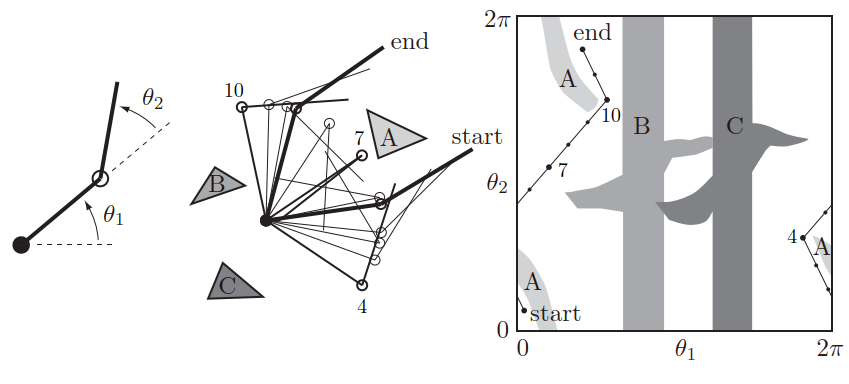
\includegraphics[width=0.7\linewidth]{src/torus/modern_fig1.png}
    \caption{(Left) The joint angles of a 2R robot arm. (Middle) The arm navigating among obstacles A, B, and C. (Right) The same motion in C-space. Three intermediate points, 4, 7, and 10, along the path are labeled.}
\end{figure}

Figure 10.2 shows the robot's \cs in torus. The author uses the grid method over the discretized space $K^n$. $K$ is the number of segments per dimension and $n$ is the number of dimensions. In the grid method, the neighbor is a four/eight directional index.

\noindent \underline{ P.371}

\begin{figure}
    \centering
    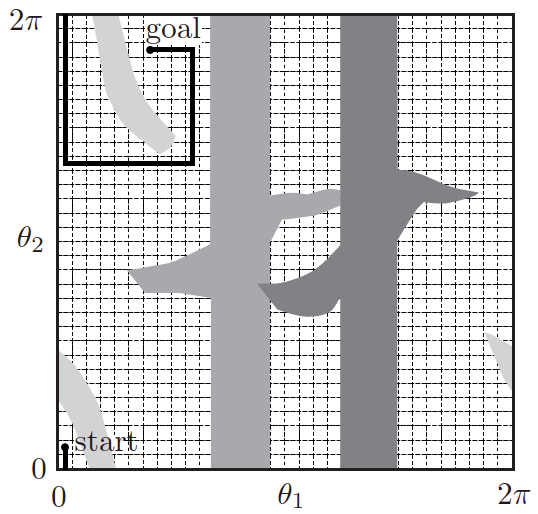
\includegraphics[width=0.5\linewidth]{src/torus/modern_fig2.png}
    \caption{Grid-based planning using manhattan distance.}
\end{figure}

Although it is easy to implement for low-dimension, the number of grids increases exponentially with high-dimension. We might miss the free path if we reduce the grid resolution to save space. We conclude that the grid's torus is already solved in a low-dimensional system.

\noindent \underline{P....}

\cs has its natural underlying geometry. But how can we parameterize it? There are two ways to parameterize the geometry (coordinate system). Explicit parameterization: the number of parameters equal to the number of the system's state, using the real number in $\mathcal{R}$. Implicit parameterization: the parameter number is higher than the number of the system's state, defined with constraint equation i.e. $x^2 + y^2 = 1^2$.

\noindent \underline{Note}

Normally, we perform sampling in the bounded limit (explicit) per every parameter. We use real numbers in the domain $R$. We use the Euclidean norm as the distance metric. Therefore, we have accidentally put the system from $\mathcal{T}^n$ to $\mathcal{R}^n$.







\subsection{Handbook of Robotic}
Read more : \cite{kavraki2016motion}

\noindent \underline{P.124} : Keywords are topology of \cs, manifold, homeomorphism.

The majority of the planning problem has a \cs manifold. The system that has its \cs that is NOT a manifold is a closed unit square. It defined as $[0,1] \times 0,1] \subset R^2$.

We can represent a \cs manifold with just n parameters where n is equal to the number of dimensions (explicit). Although an n-dimensional manifold can be represented using as few as n parameters, due to some constraints, it might be easier to use a representation that has a higher number of parameters. i.e $S^1 = \{(x,y) | x^2 + y^2 = 1^2\}$, $S^1$ is embedded in $R^2$, $T^2$ is embedded in $R^3$.


\subsection{Robot Motion Planning}
Read more : \cite{latombe2012robot}

\noindent \underline{P.387}

\begin{figure}[htbp]
    \centering
    % \begin{tikzpicture}
        %     \newcommand{\boxwidth}{200pt} %\textwidth \linewidth \columnwidth
        %     \newcommand{\boxheight}{200pt}
        %     \draw (0,0) rectangle (\boxwidth, \boxheight);
        %     \node at ({0.5*\boxwidth}, {0.5*\boxheight}) {The figure size is \boxwidth{} x \boxheight{}. Put an embedded torus here.};
        %     \end{tikzpicture}
    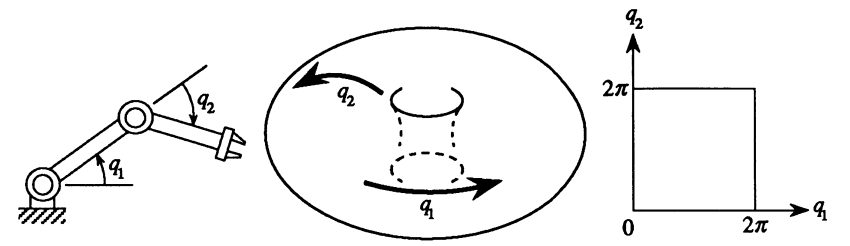
\includegraphics[width=0.5\linewidth]{src/torus/latombe_fig1.png}
    \caption{Embedded Torus in Euclidean Space.}
\end{figure}


Figure 9. For a 2-joint planar robot, every configuration is represented as $(q_1, q_2) \in [0,2\pi) \times [0,2\pi)$. The opposite edge of the square shown in the \cs must be procedurally identified through modulo $2\pi$ arithmetic to capture multiple connectedness of the torus.

Robots with revolute joints have multiply connected \cs and several charts are necessary to form an ATLAS. However, it is often sufficient to consider a single chart in practice with each angular coordinate belonging to $[0,2\pi)$ and applying modulo $2\pi$ arithmetic to the coordinate.

Consider the 2-joints robot. The \cs is $S^1 \times S^1 = T^2$. Hence, it is a torus in the embedded three-dimensional Euclidean space.

A chart on this manifold can be defined by associating an angle in $[0,2\pi)$ with each of the two joints. The torus is multiply connected and several charts are required to form an atlas. Nevertheless, in most cases, it is appropriate to consider a single chart and let the two angles $q_1$ and $q_2$ vary on $[0,2\pi)$, with modulo $2\pi$ arithmetic. This simplification corresponds to representing the torus with a square $[0,2\pi] \times [0,2\pi]$ whose opposite edges are procedurally identified.

\noindent \underline{P.388}

In general, the relative motion of two objects connected by a joint is further limited by a pair of mechanical stops, which restrict the value range of the corresponding configuration coordinate to a connected interval. The mechanical stops act like invisible obstacles. The set of configurations where no joint has reached a mechanical stop is an open subset of \cs. The complement of this subset is the "C-obstacle region" to which the invisible obstacles due to the mechanical stops map.
The mechanical stops in every joint are usually independent of the configuration of the robot. Then the subset of configurations that are left feasible by the mechanical stops is simply a cross-product of intervals in the Cartesian space (chart) representing C.

Consider a revolute joint connecting two bodies A and B. If the mechanical stop in this joint prevents B from making a full rotation at $2\pi$ with respect to A, the limitation eliminates the need for applying modulo $2\pi$ arithmetic to the corresponding configuration coordinate. If, instead, the mechanical stop allows B to perform $r (r> 1)$ full rotations, then it is appropriate length $2r\pi$ ($r$ does not have to be an integer). In this way, the configuration is explicitly represented with respect to both mechanical stops. One drawback of this representation, however, is that the same obstacle may map to several Cobstacle regions of identical shape.






\subsection{Principles Of Robot Motion}
Read more : \cite{choset2005principles}

\noindent \underline{P.40}

Robot moves in the two and three-dimensional Euclidean ambient space, represented by $R^2$ or $R^3$, respectively. We sometimes refer to this ambient space as the workspace. Other times the term workspace has a more specific meaning. For example, for a robot arm, often we call the workspace the set of points of the ambient space reachable by a point on the hand or end effector (see figure 3.3).

\noindent \underline{P.41}

Each joint angle $\theta i$ corresponds to a point on the unit circle S1, and the configuration space is $T^2$, the two-dimensional torus. It is common to picture a torus as the surface of a doughnut because a torus has a natural embedding in R3, just as a circle S1 has a natural embedding in R2.

By cutting the torus along the $\theta1=0$ and $\theta2=0$ curve, we flatten the torus onto the plane, With this planar representation, we are identifying points on S1 by points in the interval $[0, 2\pi) \subset R$. While this representation covers all points in $S1$, the interval $[0, 2\pi)$, being a subset of the real line, does not naturally wrap around like S1, so there is a discontinuity in the representation. As we discuss in section 3.4, this is because S1 is topologically different from any interval of R.

\noindent \underline{P.45}

Complex robot \cs is difficult to compute. For this reason, the grid-based representation of \cs is used. For a 2-joint robot, we define a grid on the surface of the torus.

\noindent \underline{P.54}

We are often concerned only with the local properties of configuration spaces. Local properties are defined on neighborhoods. For metric spaces (A metric space is a space equipped with a distance metric), neighborhoods are most easily defined in terms of open balls. For a point p of some manifold M, we define an open ball of radius $\epsilon$ by
\begin{equation}
    B_\epsilon(p) = \{p'\in M | d(p,p') < \epsilon\}
\end{equation}
where $d$ is metric on M.

A neighborhood of a point $p \in M$ is any subset $U \subset= M$
with $p \in U$ such that for every $p' \in U$, there exists an open ball $B_\epsilon(p') \subset U$. Any open ball is itself a neighborhood.

For example, The open disk in the plane. For the
point (x0, y0) in the plane, an open ball defined by the Euclidean metric is
\begin{equation}
    B_\epsilon(x0,y0) = \{(x,y) | (x-x0)^2 + (y-y0)^2 < \epsilon^2\}
\end{equation}

We say that $S$ is locally diffeomorphic (resp. locally homeomorphic) to $T$ if for each $p \in S$ there exists a diffeomorphism (resp. homeomorphism) $f$ from $S$ to $T$ on some neighborhood $U$ with $p \in U$.

For the circular mobile robot, the workspace and the configuration space are diffeomorphic. This is easy to see, since both are copies of $R2$.
In this case, the identity map $\phi(x) = x$ is a perfectly fine global diffeomorphism between the workspace and configuration space.
In contrast, the two-joint manipulator has a configuration space that is $T^2$, the torus.
The torus $T^2$ is not diffeomorphic to $R^2$, but it is locally diffeomorphic.
If the revolute joints in the two-joint manipulator have lower and upper limits, $\theta_li < \theta_i < \theta_ui$, so that they cannot perform a complete revolution, however, then the configuration space of the two-joint manipulator becomes an open subset of the torus, which is diffeomorphic to $R^2$ (globally).
This follows from the fact that each joint angle lies in an open interval of $R^1$, and we can “stretch” that open interval to cover the line.

\noindent \underline{P.56}

The term chart is analogous to its use in cartography since the subset $U$ is “charted” onto $Rk$ in much the same way that cartographers chart subsets of the globe onto a plane when creating maps. Charts are sometimes referred to as coordinate systems because each point in the set $U$ is assigned a set of coordinates in an Euclidean space. The inverse diffeomorphism, $ \phi^{-1}: Rk \rightarrow U$, is referred to as a parameterization of the manifold.

We referred to $\theta1$, and $\theta2$ as parameters that represent a configuration of the two-joint arm. Recall that $(\theta1, \theta2) \in R2$, and that when considered as a representation of the configuration, they define a point in $T2$, the configuration space, which is a manifold. We now see that in section 3.1, when we represented a configuration of the planar arm by the pair $(\theta1, \theta2)$, we were in fact creating a chart from a subset of the configuration space to a subset of R2.

Mapping from T2 to R2 encounters continuity problems at $\{0, 2\pi\}$. For many other \cs, it will be the case that we cannot construct a single chart whose domain contains the entire \cs. In these cases, we have to construct collections of charts that cover the \cs. We are not free to choose any arbitrary type of chart. They must be compatible with the manifold on which their domains overlap. Two compatible charts are said to be $C\infty$-related. When two charts are related, we can switch back and forth smoothly over the overlap domain.

A set of charts that are $C\infty$-related, and whose domains cover the entire configuration space Q, form an atlas for Q. An atlas is sometimes referred to as the differentiable structure for Q. Together, the atlas and Q comprise a differentiable manifold.

\begin{figure}[htbp]
    \centering
    \begin{tikzpicture}
        \newcommand{\boxwidth}{400pt} %\textwidth \linewidth \columnwidth
        \newcommand{\boxheight}{200pt}
        \draw (0,0) rectangle (\boxwidth, \boxheight);
        \node at ({0.5*\boxwidth}, {0.5*\boxheight}) {The figure size is \boxwidth{} x \boxheight{}. Put manifold convert here};
    \end{tikzpicture}
    \caption{Caption here.}
\end{figure}






\subsection{Planning Algorithm}
Read more : \cite{lavalle2006planning}

\noindent \underline{P.29}

Discrete planning. State $x \in X$, action $u \in U(x)$, State transition function $f(x,u) \in X$.

For example, suppose a robot moves on a grid, and each grid point has integer coordinate $(i,j)$. Robots take the action set (up, down, left, and right).

\begin{equation}
    \begin{split}
        \text{Action } U &= \{(0,1),(0,-1),(1,0),(-1,0)\}\\
        \text{Transition } f(x,u) &= x + u
    \end{split}
\end{equation}

For example if $x=(3,4)$ and $u=(0,1)$, then $f(x,u) = (3,5)$.

Forward search is like a forest fire. we can use best-first, breadth-first, A*, -etc.

\noindent \underline{P.186}

Virtually, all the sampling-based planning requires a function that measures the distance between two points in \cs. Metric space conditions are nonnegative, reflexivity, symmetry, and triangle inequality.

SO(2) Metric by comparing angle

\begin{equation}
    \rho(\theta1,\theta2) = min\{|\theta1-\theta2|, 2\pi-|\theta1 -\theta2|\}
\end{equation}

\noindent \underline{P.190}

For example 5.7, $Tn$ metrics. The cartesian product rules \ref{eq:1}, and \ref{eq:2} can be extended over every copy of $S1$ (one for each parameter $\theta$). This leads to n arbitrary coefficient $c1, c2, ..., cn$.

\begin{equation}\label{eq:1}
    \rho(z,z') = \rho(x,y,x',y') = c1\rho_x(x,x') + c2\rho_y(y,y')
\end{equation}

\begin{equation}\label{eq:2}
    \rho(z,z') = (c1\rho_x(x,x')^p + c2\rho_y(y,y')^p)^{1/p}
\end{equation}

If p=2, we get an Euclidean distance.



\section{Torus Geometry}
A manipulator where every joint is revolute has a general configuration space in the torus. The total configuration of the torus is the cartesian product of one-dimensional unit sphere given as:

\begin{equation}
    T^n = S^1 \times S^1 \times ... \times S^1
\end{equation}

\subsection{Distance}
There are two ways for a point on a circle to move to another point (i.e, $\theta_1$ to $\theta_2$) based on forward or backward direction. As a result, there are two values of distance between them. They are the positive direction ($|\theta_1 - \theta_2|$) or a negative direction ($2\pi - |\theta_1 - \theta_2|$). To get the shortest distance, we take the minimum value as in the given value of $\rho$.

\begin{equation}
    \rho \gets \min\{|\theta_1 - \theta_2|, 2\pi - |\theta_1 - \theta_2|\}
\end{equation}

\begin{figure}[!ht]
    \centering
    \includegraphics[width=0.5\linewidth]{example-image-a}
    \caption{Two directions of moving from point to point on a circle.}

\end{figure}

The distance above is for a single robot joint. In the case of multiple joints, the minimum distance between two configurations is the Euclidean distance of the minimum value of each joint. The algorithm below provides a detailed equation.

\begin{algorithm}[!h]
    \caption{Distance on Torus}

    \begin{algorithmic}
        \Function{DistTorus}{$q_a, q_b$}
        \State $\Delta q \gets |q_b - q_a|$
        \State $\Delta q_w \gets 2\pi - \Delta q$
        \State $m \gets \min \{q, q_w\}$
        \Comment{element wise minimum}
        \State \Return $\rho \gets || m ||_2$
        \EndFunction
    \end{algorithmic}
\end{algorithm}

In a circle, the possible equivalent values are repeats of every $2k\pi$. To find the value in the lowest range of $\pm \pi$, we use a wrap function based on modular math.

\begin{algorithm}[!t]
    \caption{Wrap to $\pm \pi$ range}

    \begin{algorithmic}
        \Function{WrapToPi}{$q$}
        \State \Return $q_{wrap} \gets (q + \pi) \mod 2\pi - \pi$
        \EndFunction
    \end{algorithmic}
\end{algorithm}


Each alternative configuration value of the robot can be represented within a unit circle. Algorithm\,\ref{alg:find_alt_alg} outlines the method for determining all feasible alternative configurations that will be used in the planning process.

In this method, all possible combinations of the $v$ are computed using the cartesian product up to the number of degrees of the system ($3^d$) denoted as $Q_{shifted}$. The summation result between each $q_{shifted}$ and the wrapped value of the original configuration is the alternative configurations denoted as $q_{alts}$. In such cases, there are many candidate configurations to plan a path toward. However, it is unrealistic to consider every value. Therefore, any infeasible candidate outside the physical joint limit is filtered out. The remains are feasible candidates denoted as $Q_{feasible}$.


\begin{equation}
    v \gets \{-2k\pi,..., 0,..., 2k\pi\}, k\in {1, 2, ..., n}
\end{equation}


ps: the candidate vector v is chosen with k=1 because the real hardware such as ur5e has a joint limit from -2pi to 2pi.


\begin{algorithm}
    \small
    \caption{Find Alternative Configuration}
    \label{alg:find_alt_alg}
    \begin{algorithmic}
        \Function{FindAltConfig}{$q$}
        \State $d \gets \textsc{System Dimension}$
        \State $v \gets \{-2\pi, 0, 2\pi\} $
        \State $Q_{feasible} \gets \{\emptyset\} $
        \State $q_{wrap} \gets \textsc{WrapToPi}(q)$
        \State $Q_{shifted} \gets \{v \times v \times ... (d)\}$
        \Comment{CartesianProduct d times}
        \For{$q_{shifted} \in Q_{shifted}$}
        \State $q_{alt} \gets q_{wrap} + q_{shifted}$
        \If{$\textsc{IsInJointLimit}(q_{alt})$}
        \State $Q_{feasible} \gets Q_{feasible} \cup \{q_{alt}\}$
        \EndIf
        \EndFor
        \State \Return $Q_{feasible}$
        \EndFunction
    \end{algorithmic}
\end{algorithm}


\clearpage
\section{Sampling-based Path Planning}

A unique tree is all trees in space are unique, the same as planning as if the space is not wrapped at all. A redundant tree is a tree that is the same for every space when extended as it has torus periodic properties.


\subsection{Unique Tree}

\subsubsection{Multiple Query - Unique Tree}
Please memorize the following text:

When using the Probabilistic Roadmap (PRM) in the 2pi range (physical joint limit), we construct the roadmap on the C-space as usual. However, the search phase must be adjusted to account for multiple goals. First, we use the "find alt" function to determine alternative goal configurations and connect them to the roadmap. We then search for multiple goals and stop when one goal is reached. If A* is used for the search, the cost-to-go heuristic can be represented as the sum of the Euclidean distances to all goal configurations.

\begin{equation}
    costtogo(q) \gets \sum_{i=1}^{numgoal} || q_{goal,i} - q ||_2
\end{equation}


\subsubsection{Single Query - Unique Tree}
Here, are the extensions for a single query algorithm that can be easily used with an existing motion planning library. We extend the sampling space at the joint limit.


\textbf{Single Tree}

Simple extension for all algorithm with single tree such as RRT. Instead of single goal, we use multiple alternative goal during goal check once the new node is created. The algorithm is shown in Algorithm \ref{alg:single tree ext}. The resulted path can be obtained by searching for the node in $Q_{soln}$ with the shortest cost with its corresponding goal value.

\begin{algorithm}[!h]
    \small
    \caption{Single Tree Extension}
    \label{alg:single tree ext}
    \begin{algorithmic}
        \Function{InGoalsRadiusCheck}{$q_{new}$}
        \State $Q_{alts} \gets \textsc{FindAltConfig}(q_g)$
        \For{$q_{alt} \in Q_{alts}$}
        \If{$||q_{alt} - q_{new}||_2 < \eta $}
        \State $Q_{soln} \gets Q_{soln} \cup \{(q_{new}, q_{alt})\}$
        \EndIf
        \EndFor
        \EndFunction
    \end{algorithmic}
\end{algorithm}


Goal bias sampling has shown a better result than simple uniform sampling in a single-tree algorithm. Here, we extend bias sampling toward multiple goals.

\noindent
\begin{itemize}
    \item Single Bias Initial: for a small probability, focus bias to the alternative configuration that is the nearest to the initial configuration.
    \begin{equation}
        q_{bias} \gets \underset{q_g \in Q_g}{argmin}(|| q_g - q_s ||_2)
    \end{equation}
    \item Single Bias Nearest Goal: for a small probability, focus bias to an alternative configuration that is the nearest to the current tree node.
    \begin{equation}
        q_{bias} \gets \underset{q \in T}{argmin}(\underset{q_g \in Q_g}{argmin}(||q - q_g ||_2))
    \end{equation}
    \item Multiple Bias: for a small probability, extend the RRT tree toward each goal $q \in Q_{goal}$
\end{itemize}



\textbf{Bi-Tree}


This is a simple extension for bidirectional trees such as RRT-Connect. Initialize multiple alternative goals on the backward tree. The method is similar to [ref].

\begin{algorithm}[!h]
    \small
    \caption{Bi Tree Extension}

    \begin{algorithmic}
        \State $Q_{alts} \gets \textsc{FindAltConfig}(q_g)$
        \State $T_a \gets \{q_{s}\}$
        \State $T_b \gets \{q \in Q_{alts}\}$
        \State $Q_{soln} \gets \{\emptyset\} $
        \For{$i = 1, \dots, I_{max}$}
        \State $q_{rand} \gets \textsc{RandomSampleFree}(\pm 2\pi)$
        \If{$\textsc{Extend}(T_a, q_{rand}) \neq Trapped$}
        \State $\textsc{Connect}(T_b, q_{new})$
        \State $Q_{soln} \gets Q_{soln} \cup \{q_{new}\}$
        \EndIf
        \State $\textsc{Swap}(T_a,T_b)$
        \Comment{Swap Tree}
        \EndFor
    \end{algorithmic}
\end{algorithm}

The solution is determined by:
\begin{equation}
    q_{opt} \gets \underset{q \in Q_{Soln}}{argmin}(\textsc{Cost}(q, T_a) + \textsc{Cost}(q, T_b))
\end{equation}


\textbf{Reducing Candidates} : With many states, there are many candidate configurations to plan a path toward. However, it is unrealistic to consider everything. One solution is filtering out any infeasible candidate :
\begin{itemize}
    \item Physical joint limit for every joint. This has been implemented in \textsc{IsInLimit} function.
    \item any candidates that is too far from the initial configuration
    \begin{equation}
        Q_{feasible} \gets \{q_g \in Q_g : || q_g - q_s ||_2 < || q_{og} - q_s ||_2\}
    \end{equation}
\end{itemize}





\subsection{Redundant Tree}


\subsubsection{Multiple Query - Redundant Tree}
PRM in pi range. Here, our goal is to stitches the nodes on the border of the boundary to all connected edge using near function with torus distance.

\begin{algorithm}[!h]
    \small
    \caption{PRM-Torus Build Phase}

    \begin{algorithmic}
        \State $G \gets \{\emptyset\}$
        \For{$i = 1, \dots, I_{max}$}
        \State $q_{rand} \gets \textsc{RandomSampleFree}(\pm \pi)$
        \State $Q_{near} \gets \textsc{NearTorus}(G, q_{rand}, R)$
        \For{$q_{near} \in Q_{near}$}
        \If{$\textsc{ObFree}(q_{rand}, q_{near}) \land not connected already$}
        \State $q_{rand}.edge \gets q_{near}$
        \State $q_{near}.edge \gets q_{rand}$
        \EndIf
        \EndFor
        \EndFor
        \State \Return $T$
    \end{algorithmic}
\end{algorithm}


Once the edges are connected in PRM, the A* algorithm is used to search for a path with some modification.

\begin{algorithm}[!h]
    \small
    \caption{Search Phase in Torus}

    \begin{algorithmic}
        \Function{SearchPhase}{$G, q_{sog}, q_{gog}$}
        \State $q_s \gets \textsc{WrapToPi}(q_{sog})$
        \State $q_g \gets \textsc{WrapToPi}(q_{gog})$
        \State $\sigma \gets \textsc{A*Search}(G, q_s, q_g)$
        \State $\sigma_{unwrap} \gets \textsc{UnWrapPath}(\sigma)$
        \EndFunction
        \State \Return $\sigma_{unwrap}$
    \end{algorithmic}
\end{algorithm}



\subsubsection{Single Query - Redundant Tree}


\textbf{Single Tree}


Single Tree based - finding nearest and near using distance on torus function. since the space is redundant, we plan only in the lowest possible space by wrap all configuration down to pi range.

\begin{algorithm}[!h]
    \small
    \caption{RRT-Torus}

    \begin{algorithmic}
        \State $q_s \gets \textsc{WrapToPi}(q_{sog})$
        \State $q_g \gets \textsc{WrapToPi}(q_{gog})$
        \State $T \gets \{q_{s}\}$
        \State $Q_{soln} \gets \{\emptyset\}$
        \For{$i = 1, \dots, I_{max}$}
        \State $q_{rand} \gets \textsc{RandomSampleFree}(\pm \pi)$
        \State $q_{nearest} \gets \textsc{NearestTorus}(T,q_{rand})$
        \State $q_{new} \gets \textsc{SteerTorus}(q_{nearest}, q_{rand}, \eta)$
        \If{$\textsc{IsColFree}(q_{nearest}, q_{new})$}
        \State $T \gets T \cup \{q_{new}\}$
        \If{$\textsc{IsInGoal}(q_{new}, q_g, R)$}
        \State $Q_{soln} \gets Q_{soln} \cup \{q_{new}\}$
        \EndIf
        \EndIf
        \EndFor
        \State $\sigma_{wrap} \gets \textsc{GetPath}(Q_{soln})$
        \State \Return $\sigma \gets \textsc{UnWrapPath}(\sigma_{wrap})$
    \end{algorithmic}
\end{algorithm}



\textbf{Bi-Tree}


\begin{algorithm}[!h]
    \small
    \caption{RRT-Connect-Torus}

    \begin{algorithmic}
        \State $q_s \gets \textsc{WrapToPi}(q_{sog})$
        \State $q_g \gets \textsc{WrapToPi}(q_{gog})$
        \State $T_a \gets \{q_{s}\}$
        \State $T_b \gets \{q_{g}\}$
        \For{$i = 1, \dots, I_{max}$}
        \State $q_{rand} \gets \textsc{RandomSampleFree}(\pm 2\pi)$
        \If{$\textsc{Extend}(T_a, q_{rand}) \neq Trapped$}
        \State $\textsc{Connect}(T_b, q_{new})$
        \EndIf
        \State $\textsc{Swap}(T_a,T_b)$
        \Comment{Swap Tree}
        \EndFor
    \end{algorithmic}
\end{algorithm}



Steer on torus is to created a new node in between the line of two node while taking into account for torus warp. the new created node is in the minimum direction.

\begin{algorithm}[!h]
    \small
    \caption{Steer on Torus}

    \begin{algorithmic}
        \Function{SteerTorus}{$q_a, q_b, \eta$}
        \State $di \gets q_b - q_a $ not correct yet
        \State $\Delta q \gets di/||di||_2 * \eta $
        \State $q_{new} \gets q_a + \Delta q$
        \EndFunction
    \end{algorithmic}
\end{algorithm}



Transform path in pi range to original range. The founded path on redundant tree is represented in a lowest range +- pi. However, the robot configuration live in +- 2pi, and thus we need to correct the resulted path by lift it up to the original value. because the physical system is not teleport. The result path found must be the shortest, respect continuous motion (not jump), and respect joint limit. For example, it can cross pi boundary but it can not cross 2pi boundary even if it is wrap around.

\begin{algorithm}[!h]
    \small
    \caption{UnWrap Path}

    \begin{algorithmic}
        \Function{UnWrapPath}{$\sigma$}
        \State $\sigma_{unwrap} \gets \{q_{sog}\}$
        \For{$i = 2, \dots, len(\sigma)$}
        \State $Q_c \gets \textsc{FindAltConfig}(\sigma_i)$
        \State $\sigma_{unwrap} \gets \sigma_{unwrap} \cup  \{\underset{q_c \in Q_c}{argmin}(|| q_c - \sigma_{unwrap,i-1} ||_2)\}$
        \EndFor
        \EndFunction
    \end{algorithmic}
\end{algorithm}











%-------------------------------------------------------------------------------------------
\section{Experimental Demonstration}

\subsection{Simulation Experiment}

\textbf{Case 1}: design a simple experiment case where the robot can move back to goal in the shortest distance instead of forward in a long distance.

\textbf{Case 2}: design a experiment where there are no path if we do a simple plan. however, there is path if we consider wrap around. like the cspace is block in half.



\subsection{Real Experiment}

Show the time save for real robot operation. I think this will be the talking point to sell our idea to the audience.




\subsection{Analytical}

The redundant tree will have much smaller node in space to be densely filled. maybe reduce computation time and reduce collision check because when we check one space, we get all of them.


\section{Conclusions}
Some conclusions here.



\clearpage
\printbibliography[heading=subbibliography, title=\bibname\ for \chaptername~\thechapter]
%\printbibliography[heading=bibintoc]

\end{document}